% Options for packages loaded elsewhere
\PassOptionsToPackage{unicode}{hyperref}
\PassOptionsToPackage{hyphens}{url}
%
\documentclass[
]{book}
\usepackage{lmodern}
\usepackage{amssymb,amsmath}
\usepackage{ifxetex,ifluatex}
\ifnum 0\ifxetex 1\fi\ifluatex 1\fi=0 % if pdftex
  \usepackage[T1]{fontenc}
  \usepackage[utf8]{inputenc}
  \usepackage{textcomp} % provide euro and other symbols
\else % if luatex or xetex
  \usepackage{unicode-math}
  \defaultfontfeatures{Scale=MatchLowercase}
  \defaultfontfeatures[\rmfamily]{Ligatures=TeX,Scale=1}
\fi
% Use upquote if available, for straight quotes in verbatim environments
\IfFileExists{upquote.sty}{\usepackage{upquote}}{}
\IfFileExists{microtype.sty}{% use microtype if available
  \usepackage[]{microtype}
  \UseMicrotypeSet[protrusion]{basicmath} % disable protrusion for tt fonts
}{}
\makeatletter
\@ifundefined{KOMAClassName}{% if non-KOMA class
  \IfFileExists{parskip.sty}{%
    \usepackage{parskip}
  }{% else
    \setlength{\parindent}{0pt}
    \setlength{\parskip}{6pt plus 2pt minus 1pt}}
}{% if KOMA class
  \KOMAoptions{parskip=half}}
\makeatother
\usepackage{xcolor}
\IfFileExists{xurl.sty}{\usepackage{xurl}}{} % add URL line breaks if available
\IfFileExists{bookmark.sty}{\usepackage{bookmark}}{\usepackage{hyperref}}
\hypersetup{
  pdftitle={Using LANDFIRE Products to explore historical and current ecosystems},
  pdfauthor={Draft by The Nature Conservancy's LANDFIRE team},
  hidelinks,
  pdfcreator={LaTeX via pandoc}}
\urlstyle{same} % disable monospaced font for URLs
\usepackage{longtable,booktabs}
% Correct order of tables after \paragraph or \subparagraph
\usepackage{etoolbox}
\makeatletter
\patchcmd\longtable{\par}{\if@noskipsec\mbox{}\fi\par}{}{}
\makeatother
% Allow footnotes in longtable head/foot
\IfFileExists{footnotehyper.sty}{\usepackage{footnotehyper}}{\usepackage{footnote}}
\makesavenoteenv{longtable}
\usepackage{graphicx,grffile}
\makeatletter
\def\maxwidth{\ifdim\Gin@nat@width>\linewidth\linewidth\else\Gin@nat@width\fi}
\def\maxheight{\ifdim\Gin@nat@height>\textheight\textheight\else\Gin@nat@height\fi}
\makeatother
% Scale images if necessary, so that they will not overflow the page
% margins by default, and it is still possible to overwrite the defaults
% using explicit options in \includegraphics[width, height, ...]{}
\setkeys{Gin}{width=\maxwidth,height=\maxheight,keepaspectratio}
% Set default figure placement to htbp
\makeatletter
\def\fps@figure{htbp}
\makeatother
\setlength{\emergencystretch}{3em} % prevent overfull lines
\providecommand{\tightlist}{%
  \setlength{\itemsep}{0pt}\setlength{\parskip}{0pt}}
\setcounter{secnumdepth}{5}
\usepackage{booktabs}
\usepackage[]{natbib}
\bibliographystyle{plainnat}

\title{Using LANDFIRE Products to explore historical and current ecosystems}
\author{Draft by The Nature Conservancy's LANDFIRE team}
\date{2021-03-08}

\begin{document}
\maketitle

{
\setcounter{tocdepth}{1}
\tableofcontents
}
\hypertarget{this-document}{%
\chapter{This document\ldots{}}\label{this-document}}

is a technical guide DRAFTED in R-Markdown using the Bookdown package. It was created to support the ``Wrangling billions (and billons) of pixels and hundreds of ecosystem models: Making LANDFIRE products work for your landscape'' working session.

\hypertarget{landfire-for-landscape-ecosystem-assessment}{%
\chapter{LANDFIRE for landscape ecosystem assessment}\label{landfire-for-landscape-ecosystem-assessment}}

There are some basic steps in assessing the ecological situation of your landscape, including:

\begin{itemize}
\tightlist
\item
  mapping historical and current ecosystems, and the difference between the two; and further looking at representation of ecosystems inside and outside of your landscape of interest.
\item
  assessing succession classes (aka seral states) of these ecosystems, past and present
\item
  understanding natural disturbance regimes
\end{itemize}

These steps, while foundational and conceptually simple can be difficult due to a lack of data, especially when doing then at a landscape scale which often means looking across multiple land ownerships.

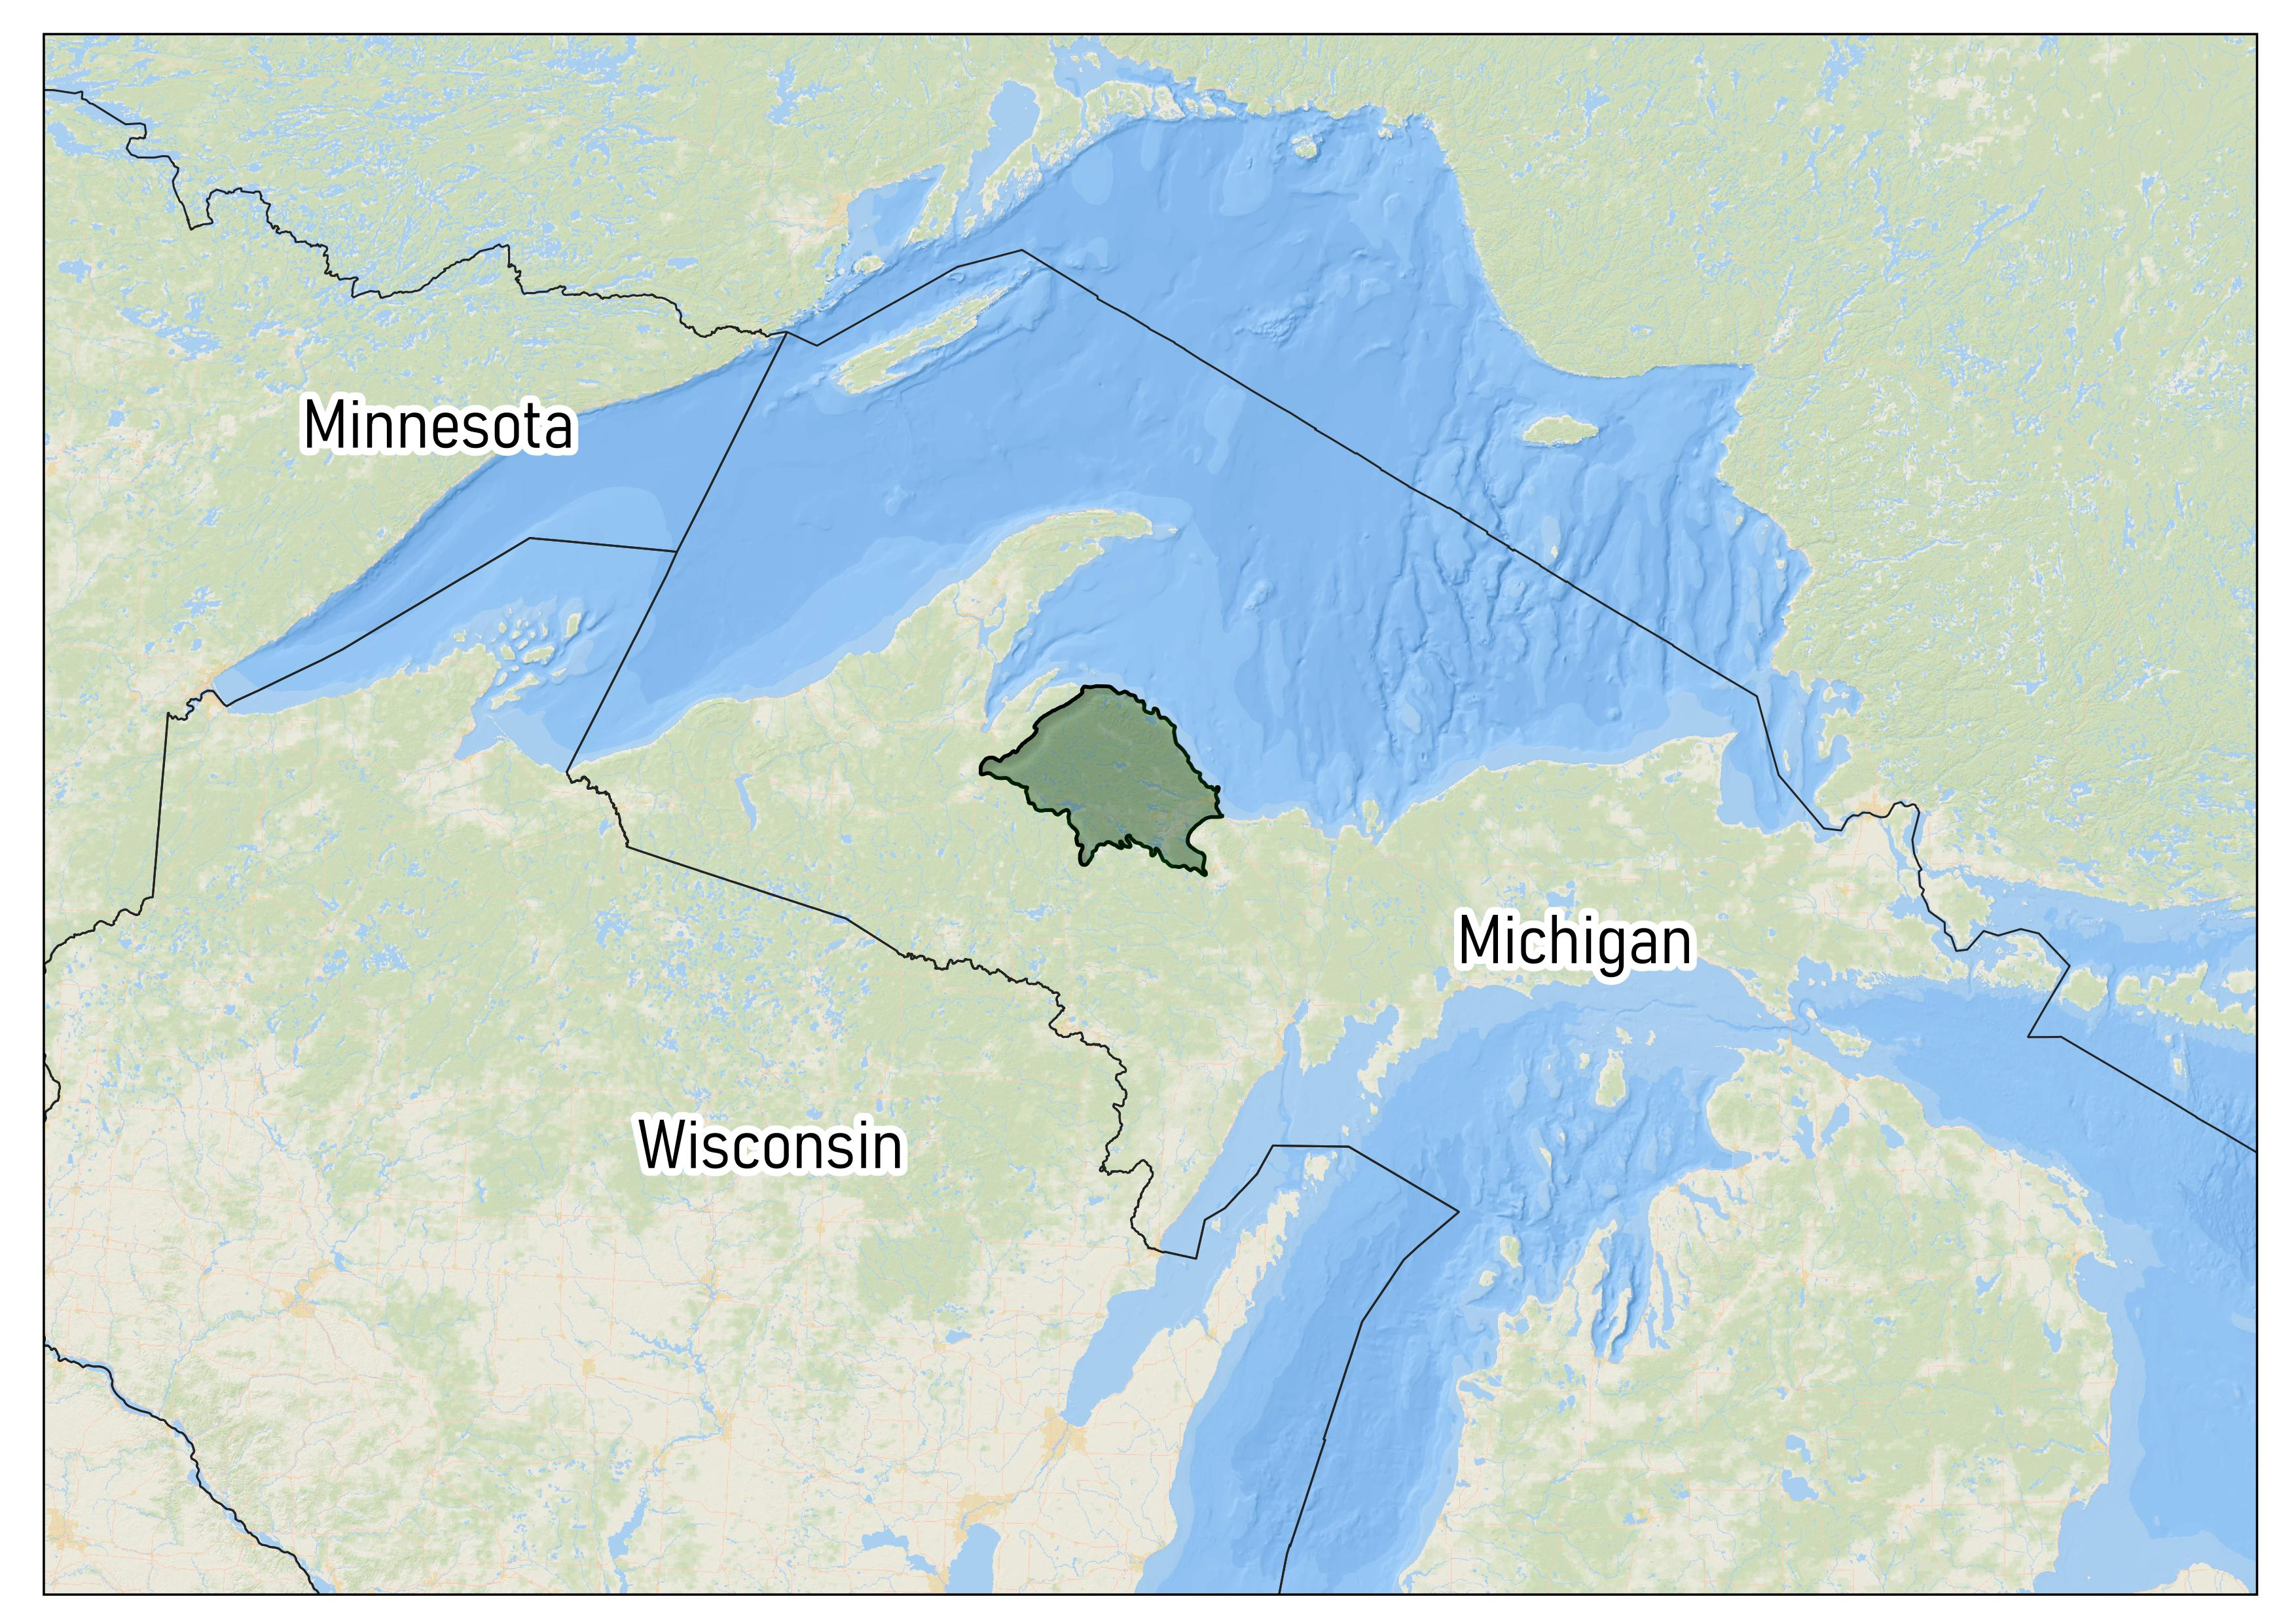
\includegraphics[width=0.5\linewidth,style="float:right; padding:10px"]{michi}

In the United States, including the insular areas \href{www.landfire.gov}{LANDFIRE} provides the datasets and ecological model results to get at these challenges and more. Here we walk you through some of the technical steps needed to start your analysis. We will do our work in a model landscape, the Michigamme Highlands in the Upper Peninsula of Michigan (highlighted in green in map).

\hypertarget{this-online-guide}{%
\section{This online guide\ldots{}}\label{this-online-guide}}

is a technical guide originally created for The Nature Conservancy's Global Science Gathering, working session titled ``Billions (and billons) of pixels coupled with hundreds of ecosystem models: Making LANDFIRE products work for your landscape''. It was written in R using R-Studio, the ``bookdown'' package and is hosted on GitHub.

\hypertarget{getting-started}{%
\section{Getting Started}\label{getting-started}}

For this guide we have done some of the heavy lifting for you, i.e., the GIS work and creation of an Excel workbook {[}\textbf{INSERT LINK HERE}{]}. You can explore the GIS work we did, and the datasets at {[}\textbf{INSERT LINK TO ARCMAP PROJECT HERE}{]}

\hypertarget{softAndData}{%
\chapter{Software and Datasets}\label{softAndData}}

\hypertarget{to-get-started-you-will-need-the-landfire-products.-the-hyperlined-text-will-lead-you-to-descriptions}{%
\section{To get started you will need the LANDFIRE products. The hyperlined text will lead you to descriptions:}\label{to-get-started-you-will-need-the-landfire-products.-the-hyperlined-text-will-lead-you-to-descriptions}}

\begin{itemize}
\tightlist
\item
  Spatial datasets, clipped to your area(s) of interest

  \begin{itemize}
  \tightlist
  \item
    \href{https://www.landfire.gov/bps.php}{Biophysical Settings (BpS)}. This dataset will be used to get at ``community habitat'', or where ecosystems could occur based on abiotic factors (e.g., soils, climate).
  \item
    \href{https://www.landfire.gov/sclass.php}{Succession classes} characterizes structural classes on the landscape at the time the dataset represents (e.g., 2016 for LF Version 200).
  \item
    \href{https://www.landfire.gov/evt.php}{Existing Vegetation Type} maps NatureServe's Ecological Systems (see descriptions \href{https://www.landfire.gov/documents/LANDFIRE_Ecological_Systems_Descriptions_CONUS.pdf}{here}).
  \end{itemize}
\item
  Non-spatial products

  \begin{itemize}
  \tightlist
  \item
    \href{http://landfirereview.org/search.php}{Biophysical Settings Descriptions} which has information on natural disturbance regimes and succession class descriptions (also available \href{https://tnc.box.com/s/d3ocvy969s1792m5885filjhktujp86e}{here}).\\
  \item
    \href{https://tnc.box.com/s/d3ocvy969s1792m5885filjhktujp86e}{Reference Condition Table} supplements the BpS descriptions with the ``reference'' percentages for each succession class, for each Biophysical Settings.
  \end{itemize}
\end{itemize}

\hypertarget{guidance-on-obtaining-landfire-products}{%
\section{Guidance on obtaining LANDFIRE products}\label{guidance-on-obtaining-landfire-products}}

There are multiple ways to get LANDFIRE depending on whether you are looking to obtain BpS models and descriptions or the spatial data:

\begin{itemize}
\item
  For BpS models and descriptions go to: \url{http://landfirereview.org/search.php}. Start by clicking on the ``View map of LANDFIRE Map Zones''. This will help you narrow down your search. Alternatively, you can wait to download BpS descriptions until you do some GIS work and get specific names of BpSs of interest.
\item
  For the spatial datasets you can explore options \href{https://www.landfire.gov/getdata.php}{here} which include:

\begin{verbatim}
  * Downloading [Full Extent Mosaics](https://www.landfire.gov/version_comparison.php).  When you do use this option you get large files that cover the entire lower 48, AK or HI (depending on your selection).  We use this method when we have several landscapes and/or a large area and no computer storage issues.
  * Using the [LANDFIRE Data Distribution Site](https://www.landfire.gov/viewer/).  With this method you essentially select the datasets you need then draw a rectangle (or you can select state or counties) around your area of interest to start the downloader.  We recommend this if your area of interest is not too large and/or you have a low number of landscapes and/or have storage limits.
\end{verbatim}
\end{itemize}

\hypertarget{historicalEcosystems}{%
\chapter{Historical Ecosystems}\label{historicalEcosystems}}

In this chapter we will learn which ecosystems, and how much of each were on our landscape historically.

\hypertarget{general-methods}{%
\section{General methods}\label{general-methods}}

In this section (and most others) we will depend on ``Pivot Tables'' in Excel. They are powerful (for better or worse!) tools that allow for tasks such as:

\begin{itemize}
\tightlist
\item
  organization and formatting of data
\item
  calculations
\item
  filtering data
\item
  nesting data
\end{itemize}

With the power comes the call for caution. It is super easy to display values that look illuminating-but may be wrong. You can easily be duped into complacency, especially when working in the ``value field settings''.

\hypertarget{getting-at-amounts-of-historical-ecosystems}{%
\section{Getting at amounts of historical ecosystems}\label{getting-at-amounts-of-historical-ecosystems}}

\textbf{Start by opening the ``historical'' tab in the Excel workbook.}

\begin{enumerate}
\def\labelenumi{\arabic{enumi}.}
\tightlist
\item
  In the Pivot Table Fields pane, select ``BPS\_NAME'' then ``ACRES''.\\
\item
  Right click in the top cell of the ``Sum of ACRES'' column (not the column header) in the Pivot Table, then ``Sort Largest to Smallest''.
\item
  In our example we have some BpSs that have low ACRES values. We also have categories that are not meaningful, such as ``Barren-Rock/Sand/Clay''. We can do a little formatting/cleaning before making a chart:

  \begin{itemize}
  \tightlist
  \item
    To remove BpSs from the table you will click the drop-down menu to the right of ``BPS\_NAME'' in the Pivot Table Fields pane. You can uncheck BpSs as appropriate.
  \item
    It is also possible to filter by right clicking on the top value in the list of BpSs, then selecting Filter \textgreater{} Top 10\ldots. Once in that menu you can refine the filtering.
  \end{itemize}
\item
  To get percentages, drag ``ACRES'' from the top Pivot Table Field pane to the ``Values'' pane. This will add a second ``ACRES'' column to the table. Click the drop down in the second instance of ``ACRES'' (reads ``SUM of ACRES2'' in our example), then Value Field Settings. In this menu select the ``Show Values As'' tab, click the ``Show Values As'' drop down then select ``\% of Grand Total\% to get percentages of each BpS (make sure that''BPS\_NAME" is selected as the ``Base field'').\\
\item
  To get a ``running total'' of percentages you will add a third instance of ``ACRES'' to the ``Values'' pane, then Value Field Settings. In this menu select the ``Show Values As'' tab, click the ``Show Values As'' drop down then select ``\% Running Total In'' to get running totals of percentages of each BpS (make sure that ``BPS\_NAME'' is selected as the ``Base field'').
\item
  Save!
\end{enumerate}

Formatted table of BpSs:

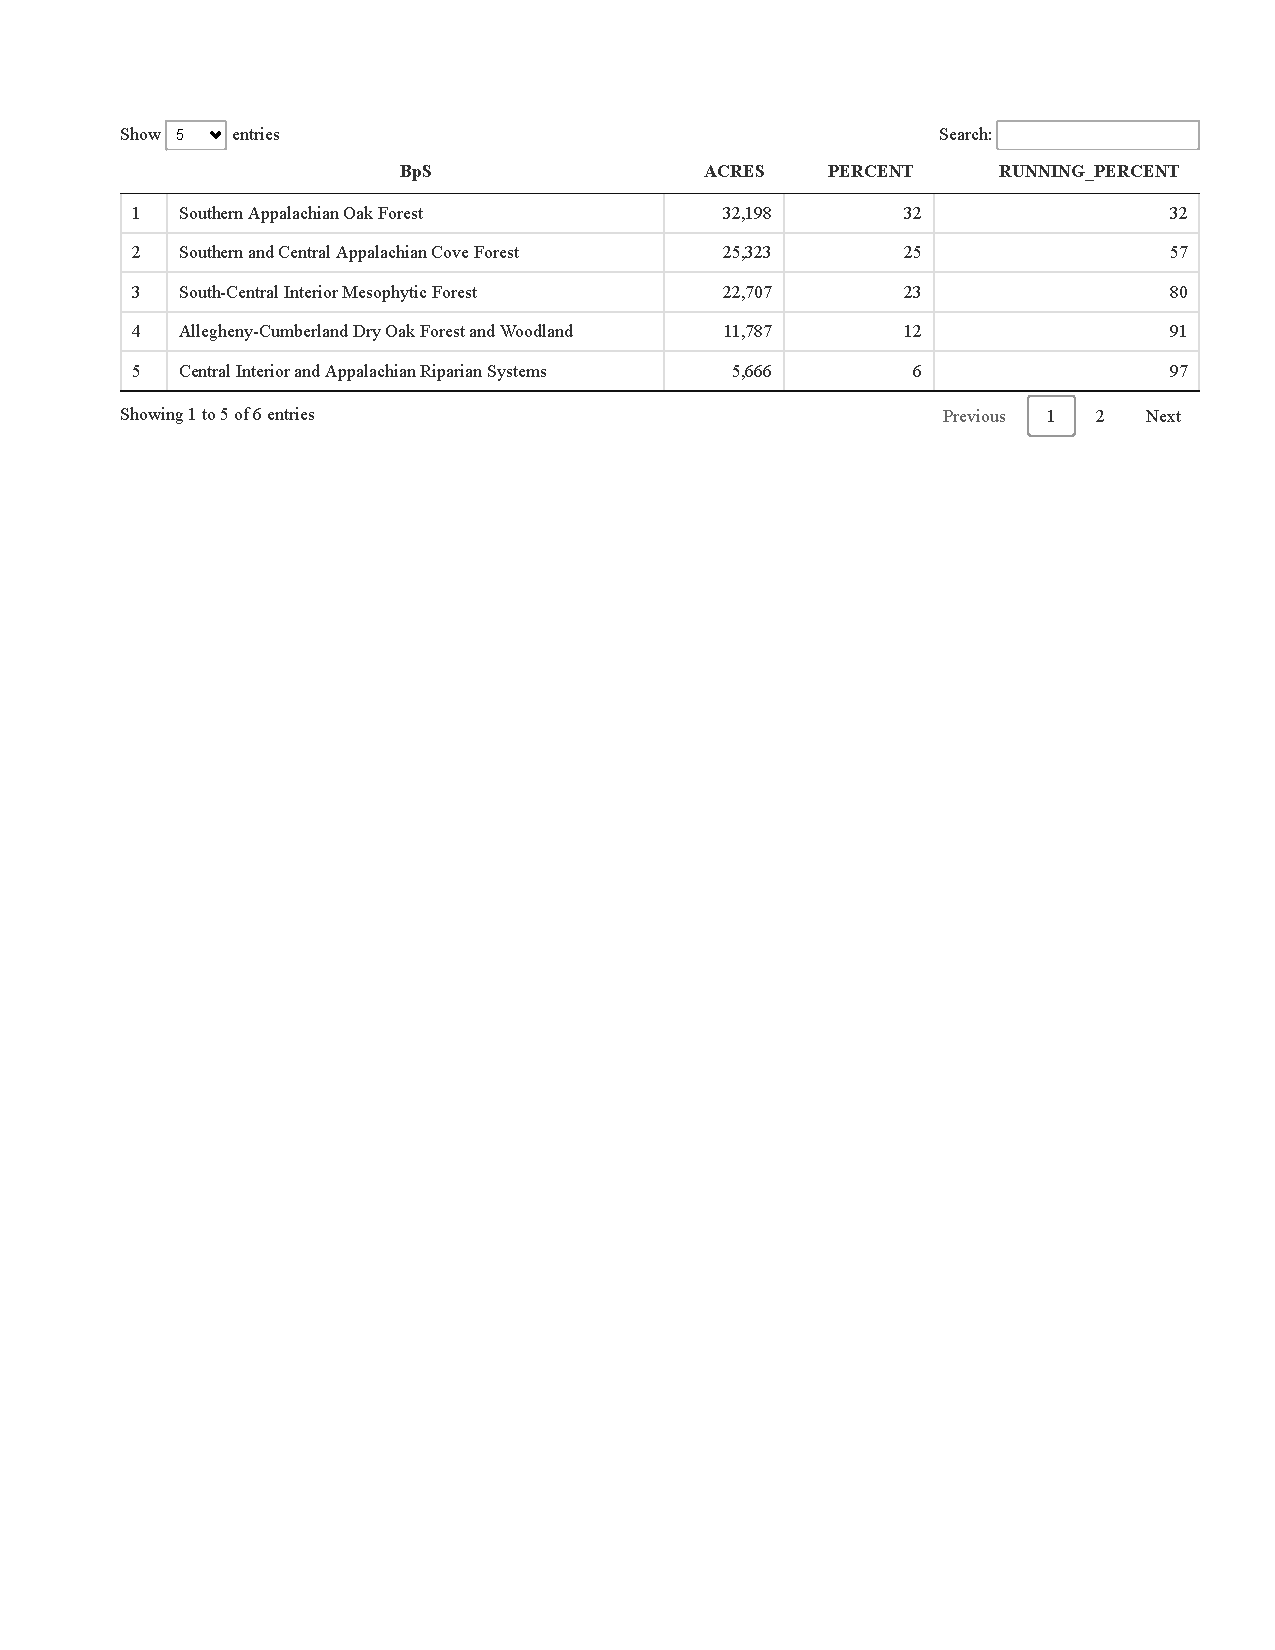
\includegraphics{FSCBook_files/figure-latex/bpsDT-1.pdf}

We see that the top 4 BpSs comprised \textasciitilde80\% of our example landscape historically. We can visually confirm this and other patterns with a quick chart made in R (similar charts available in Excel by highlighting the data, clicking Insert then selecting the chart type in the ``Charts'' tab):

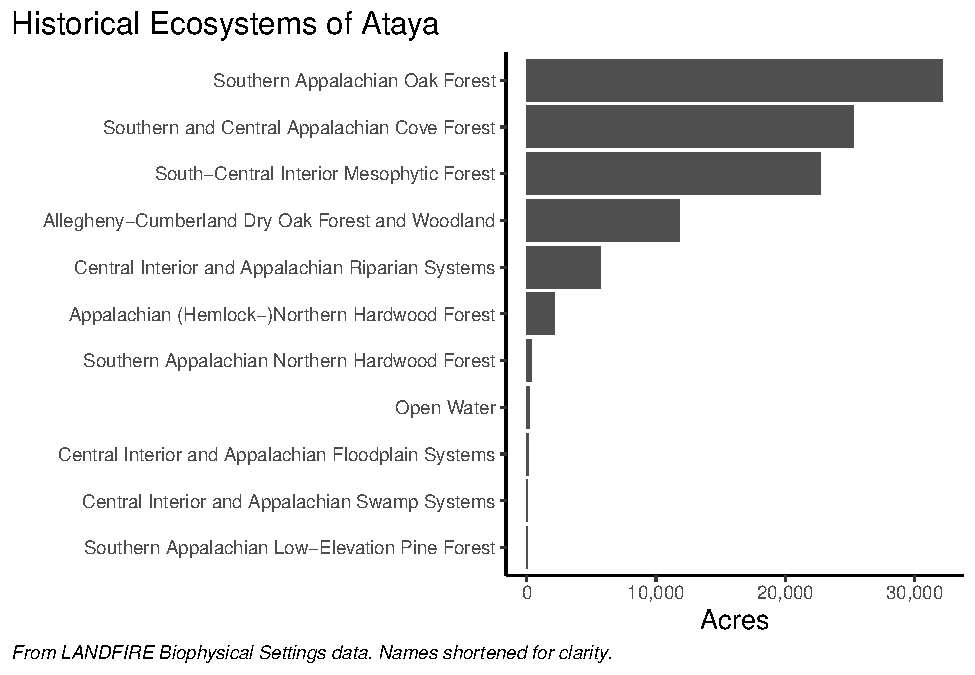
\includegraphics{FSCBook_files/figure-latex/bpsChart-1.pdf}

\hypertarget{evt}{%
\chapter{Existing Vegetation Types}\label{evt}}

While looking at the historical ecosystems gives context, we also need to get a picture of which ecosystems are on the landscape today.

\hypertarget{general-methods-1}{%
\section{General methods}\label{general-methods-1}}

We use the same general methods as we did on the ``Historical Ecosystems'' page, using a Pivot Table. We rely on \href{https://www.landfire.gov/evt.php}{LANDFIRE's Existing Vegetation Type (EVT)} data for this assessment.

\hypertarget{getting-at-amounts-of-current-ecosystems}{%
\section{Getting at amounts of current ecosystems}\label{getting-at-amounts-of-current-ecosystems}}

\textbf{Start by opening the ``current'' tab in the Excel workbook.}

\begin{enumerate}
\def\labelenumi{\arabic{enumi}.}
\tightlist
\item
  In the Pivot Table Fields pane, select ``EVT\_NAME'' then ``ACRES''. Make sure that EVT\_NAME is in the ``Rows'' pane, and that ``Sum of ACRES'' is in the ``Values'' pane.\\
\item
  Right click in the top cell of the ``Sum of ACRES'' column (not the column header) in the Pivot Table, then ``Sort Largest to Smallest''.
\item
  In our example we have some BpSs that have low ACRES values. We also have categories that are not meaningful, such as ``Barren-Rock/Sand/Clay''. We can do a little formatting/cleaning before making a chart:

  \begin{itemize}
  \tightlist
  \item
    To remove EVTs from the table you will click the drop-down menu to the right of ``BPS\_NAME'' in the Pivot Table Fields pane. You can uncheck BpSs as appropriate.
  \item
    It is also possible to filter by right clicking on the top value in the list of EVTs within the Pivot Table, then selecting Filter \textgreater{} Top 10\ldots. Once in that menu you can refine the filtering.
  \item
    Additionally we like to add commas and remove decimal places. To do this right click the row that contains ``Sum of ACRES'' in the spreadsheet (likely row ``B''), select ``Format Cells'' \textgreater{} Number \textgreater{} set Decimal places to ``0'' then check the "Use 1000 Separator box.
  \end{itemize}
\item
  To get percentages, drag ``ACRES'' from the top Pivot Table Field pane to the ``Values'' pane. This will add a second ``ACRES'' column to the table. Click the drop down in the second instance of ``ACRES'' (reads ``SUM of ACRES2'' in our example), then Value Field Settings. In this menu select the ``Show Values As'' tab, click the ``Show Values As'' drop down then select ``\% of Grand Total\% to get percentages of each BpS (make sure that''BPS\_NAME" is selected as the ``Base field'').\\
\item
  To get a ``running total'' of percentages you will add a third instance of ``ACRES'' to the ``Values'' pane, then Value Field Settings. In this menu select the ``Show Values As'' tab, click the ``Show Values As'' drop down then select ``\% Running Total In'' to get running totals of percentages of each BpS (make sure that ``BPS\_NAME'' is selected as the ``Base field'').
\item
  Save!
\end{enumerate}

Formatted table of EVTs:

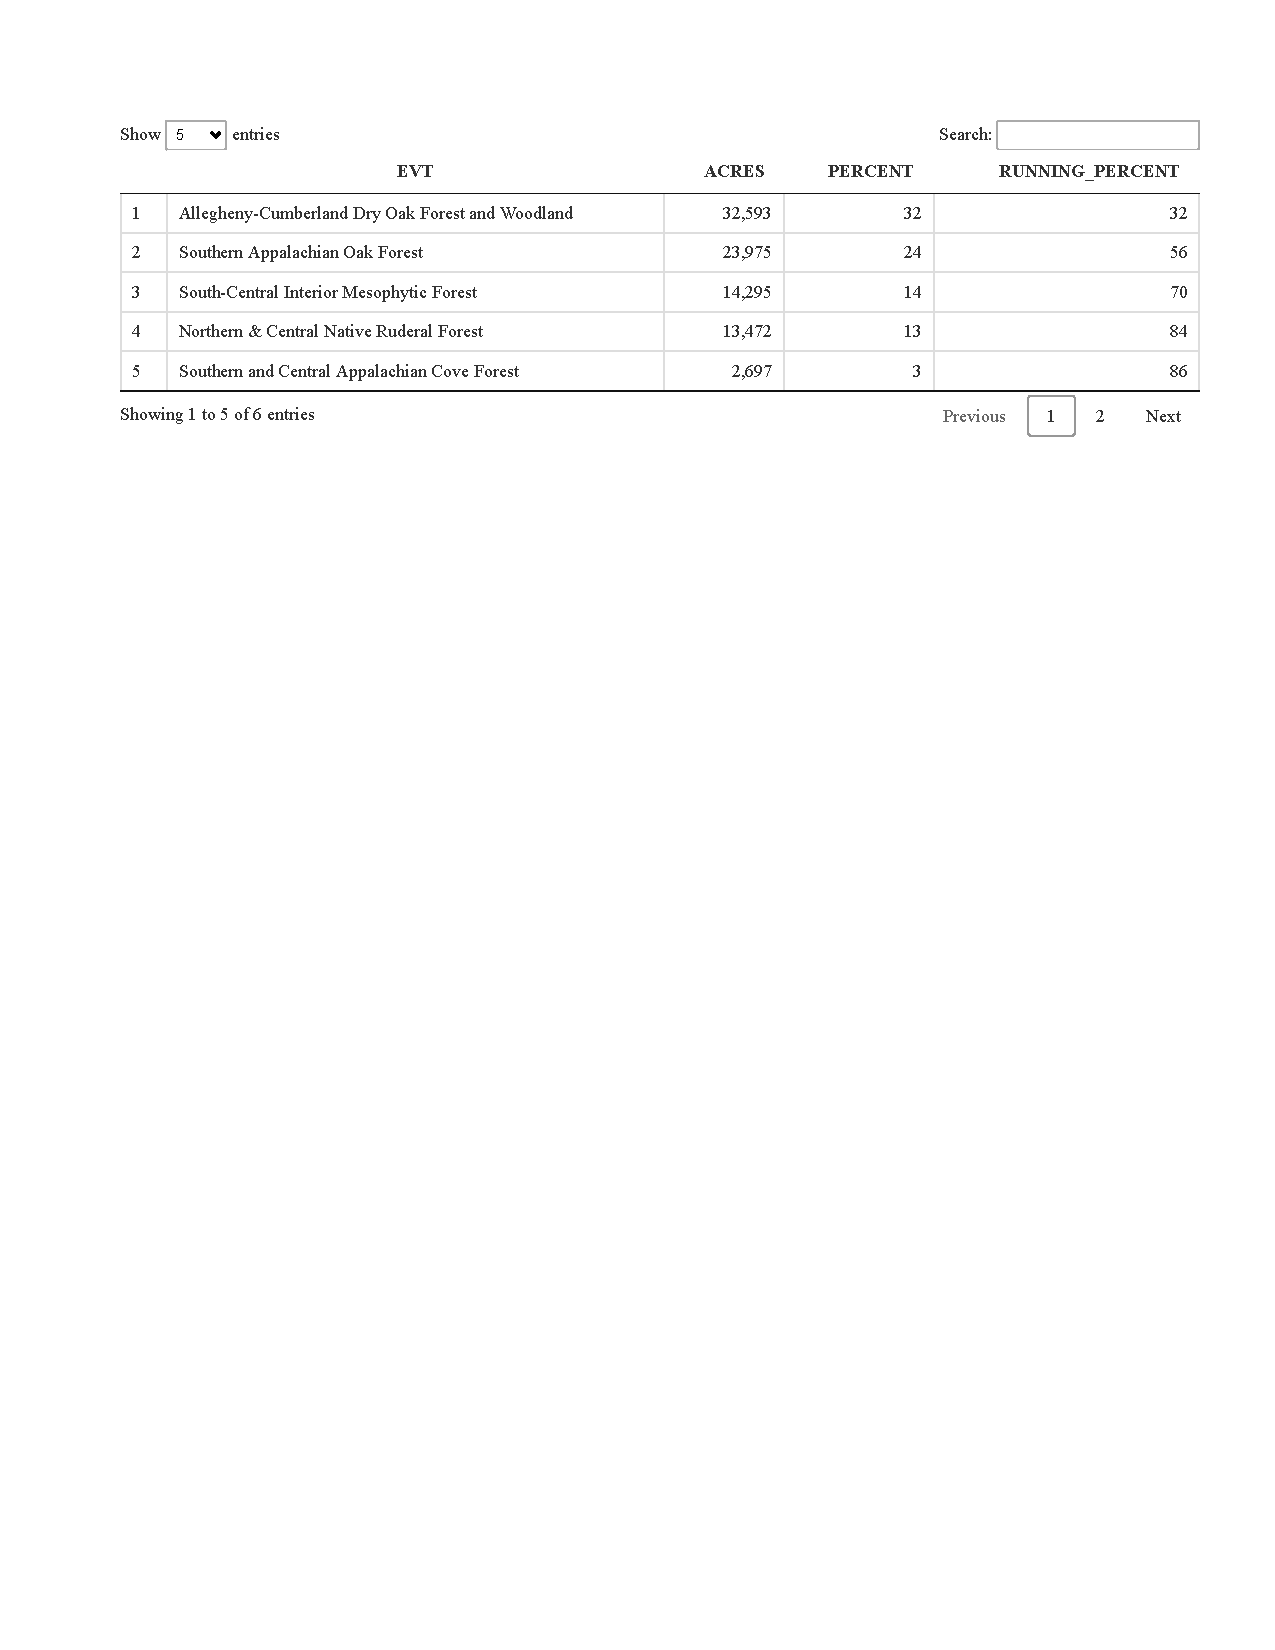
\includegraphics{FSCBook_files/figure-latex/evtDT-1.pdf}

We see that first there are many EVT's. This partially due to the addition of Developed and other ``modern'' categories such as ``Recently Logged-Tree Cover''. Second we see that of the ``natural'' types their is a close match with the historical. We can visually confirm this and other patterns with a quick chart made in R (similar charts available in Excel by highlighting the data, clicking Insert then selecting the chart type in the ``Charts'' tab):

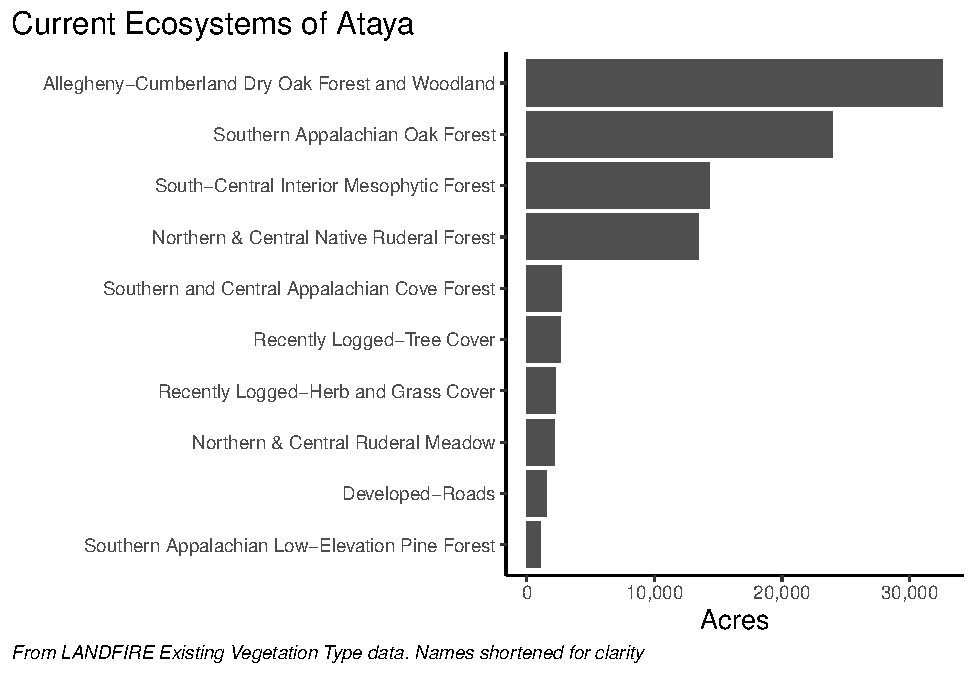
\includegraphics{FSCBook_files/figure-latex/evtChart-1.pdf}

\hypertarget{conversion}{%
\chapter{Exploring conversion}\label{conversion}}

How much have historical ecosystems been converted to other land uses, or succeeded to other ecosystem types.

\hypertarget{second-question-how-much-of-the-historic-ecosystems-have-been-converted-to-a-different-land-use-e.g.-agriculture-or-have-succeeded-to-a-different-ecosystem}{%
\section{Second question: how much of the historic ecosystems have been converted to a different land use (e.g., agriculture), or have succeeded to a different ecosystem?}\label{second-question-how-much-of-the-historic-ecosystems-have-been-converted-to-a-different-land-use-e.g.-agriculture-or-have-succeeded-to-a-different-ecosystem}}

If you are new to Pivot Tables this next section will 1) demonstrate their power and 2) showcase ways they can mislead!

Working in the Pivot Table from before (or you can create a new one if you prefer):

\begin{enumerate}
\def\labelenumi{\arabic{enumi}.}
\tightlist
\item
  Check the box next to ``EVT\_NAME'' in the Pivot Table Fields pane. Make sure that everything is arranged as in the screenshot below (e.g., ``BPS\_NAME'' is on top of ``EVT\_NAME'' in the ``Rows'' pane). Note-I am about to sort in descending order.
\end{enumerate}

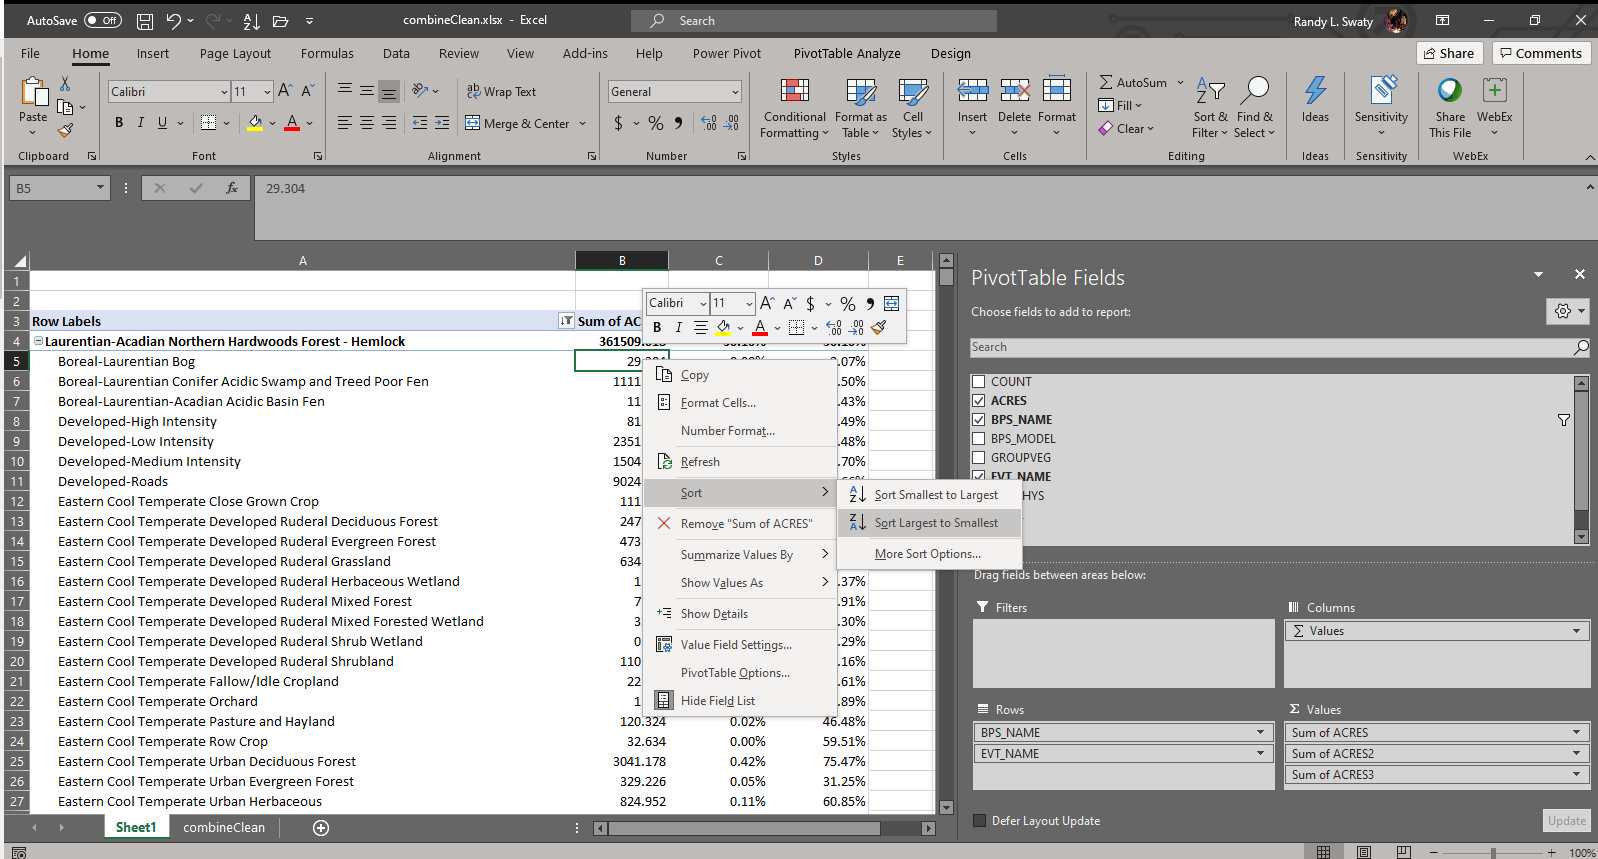
\includegraphics[width=1\linewidth]{pivotBpsEvt}

\begin{enumerate}
\def\labelenumi{\arabic{enumi}.}
\setcounter{enumi}{1}
\tightlist
\item
  Review the results. In the example above we can see that what LANDFIRE mapped as Laurentian-Acadian Forest-Hemlock in the BpS data set has been split into many Existing Vegetation Types. If ordered we get a little more information, but the numbers are misleading. We'd like to see how much of what was Ecosystem X is still Ecosystem X, and how much is now Ecosystem Y, and so on, but the numbers are looking across the whole landscape. They need to be recalculated so we get the percentage of EVT per BpS.
\item
  To reconfigure the Pivot Table:

  \begin{itemize}
  \tightlist
  \item
    Drag the ``Sum of ACRES2'' and ``Sum of ACRES3'' field from the ``Values'' pane up to the Pivot Table Fields to remove it.
  \item
    Click the ``Sum of ACRES'' item in the ``Values'' pane to access the Value field settings.
  \item
    Click on the ``Show Values As'' tab, then select ``\% of Parent Row Total'' in the ``Show Values As'' drop down.
  \end{itemize}
\end{enumerate}

Here's a screenshot of making that selection:

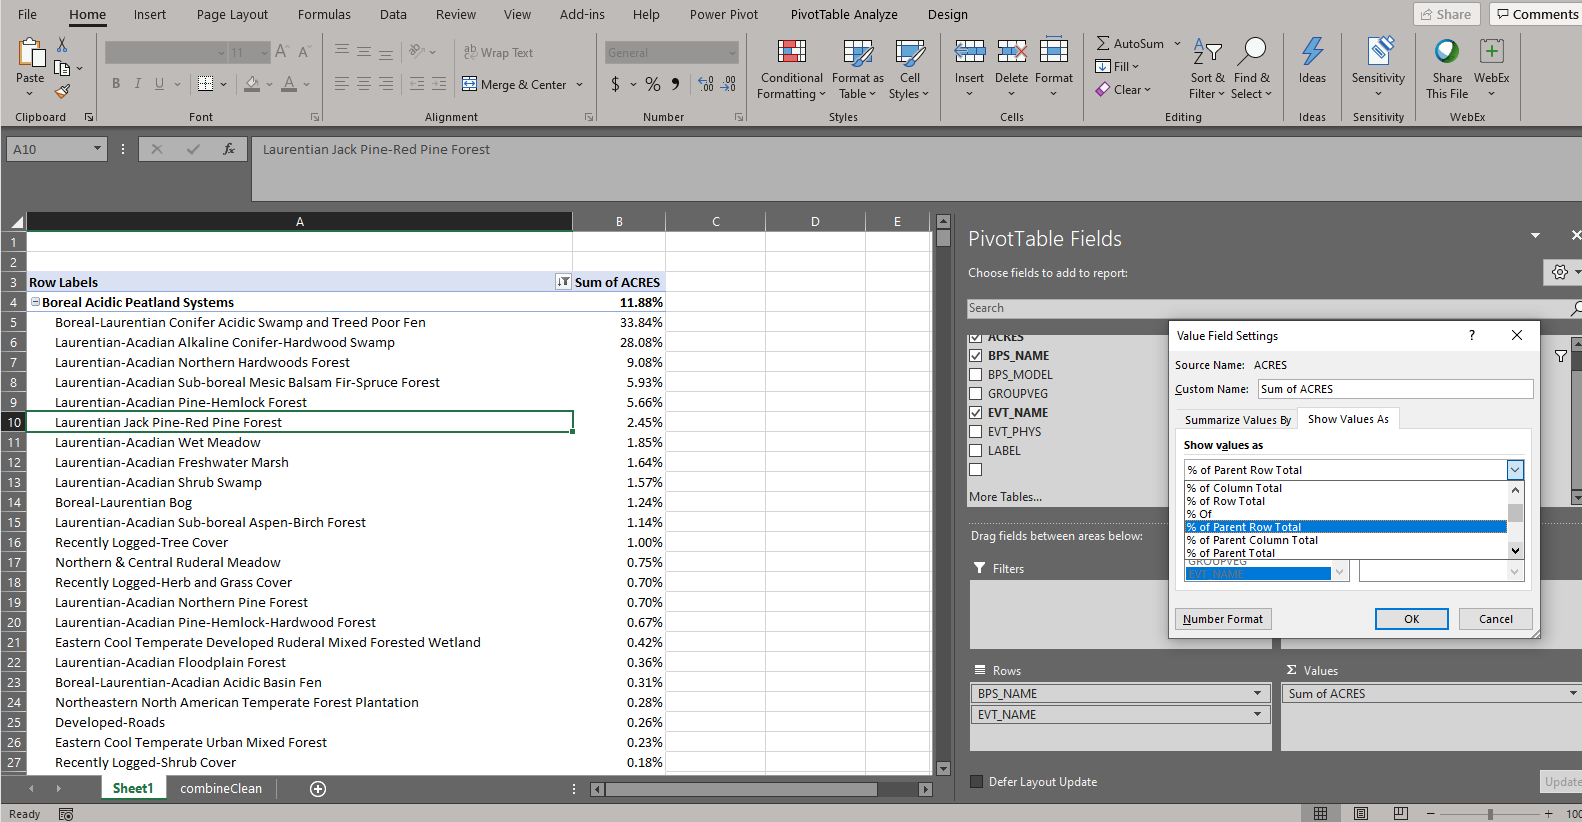
\includegraphics[width=1\linewidth]{pivotPercentParent}

You'll see that \textasciitilde34\% of what was classified as ``Boreal Acidic Peatland Systems'' in the BpS dataset for our landscape is now classified as ``Boreal-Laurentian Conifer Acidic Swamp and Treed Poor Fen'' in the Existing Vegetation Type dataset. Scroll through the table below to explore the resulting data. The table has been exported from the Pivot Table and cleaned up a bit for viewing.

\textbf{Note: I filtered for the Top 10 EVTs per BpS.}

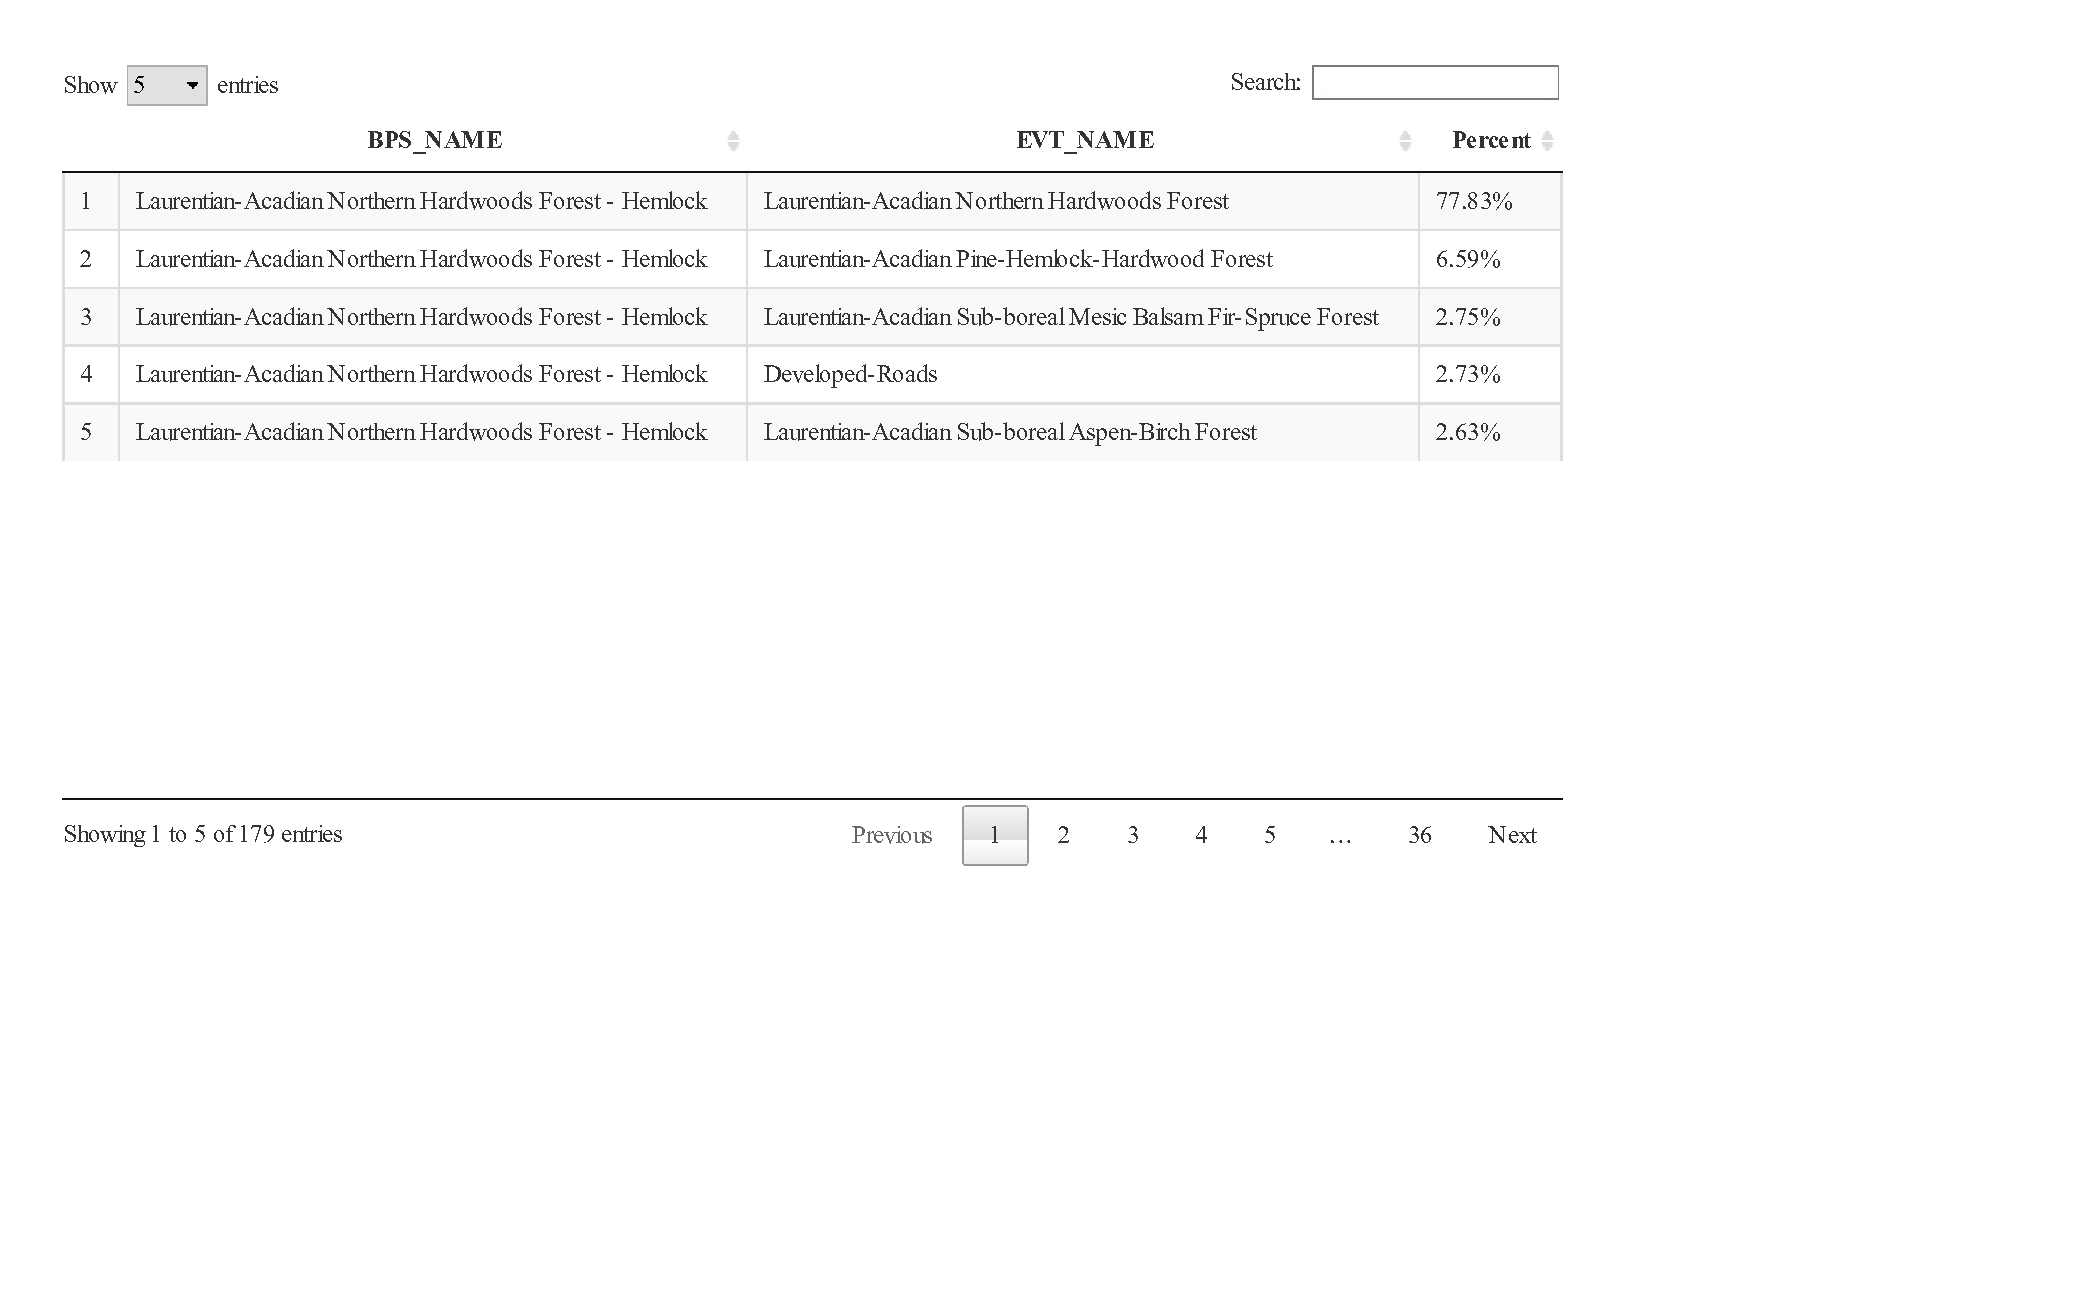
\includegraphics{FSCBook_files/figure-latex/bpsEvtDT-1.pdf}

Looking at the Laurentian-Acadian Northern Hardwoods Forest - Hemlock for our landscape we note a few things:

\begin{itemize}
\tightlist
\item
  Most of what was mapped as this type historically in the BpS dataset is still mapped as that type
\item
  Cumulatively about 6\% of this type is now roads and recently logged types.
\item
  The other EVTs mapped are not terribly ``off-site'' (e.g., something like ``Plantation'').
\end{itemize}

\hypertarget{the-fine-print}{%
\section{The fine print}\label{the-fine-print}}

While this assessment is illustrative, it is important to note that the methods used to create the BpS and EVT datasets are substantially different, and LANDFIRE datasets are not made for assessing small areas. Please review.

\hypertarget{visual-exploration}{%
\section{Visual exploration}\label{visual-exploration}}

Sometimes patterns emerge from visuals. Below is a Sankey chart generated in R. On the left are the historical ecosystems, on the right current ecosystems. If you hover over the colored bands you can explore what the historical ecosystems are today, or where current ecosystems came from. Some potential interpretations, partially based on the chart, partially based on local knowledge:

\begin{itemize}
\tightlist
\item
  There is more northern hardwoods mapped today than historically. This could be due to ``simplification'' of ecosystems that have some shared species. For example, many conifers have been removed and deer present a challenge for regeneration. One hypothesis would be that due to logging and deer the ``Pine-Hemlock-Hardwood-Forest'' has been essentially converted to ``Northern Hardwoods''.
\item
  It might be more illuminating to group some types together, such as the ``Recently Logged'' types.
\item
  LANDFIRE has mapped potential change of the wetlands to other types. This could be due to mapping errors, or due to alterations in hydrology because of roads perhaps. More investigation is warrented.
\end{itemize}

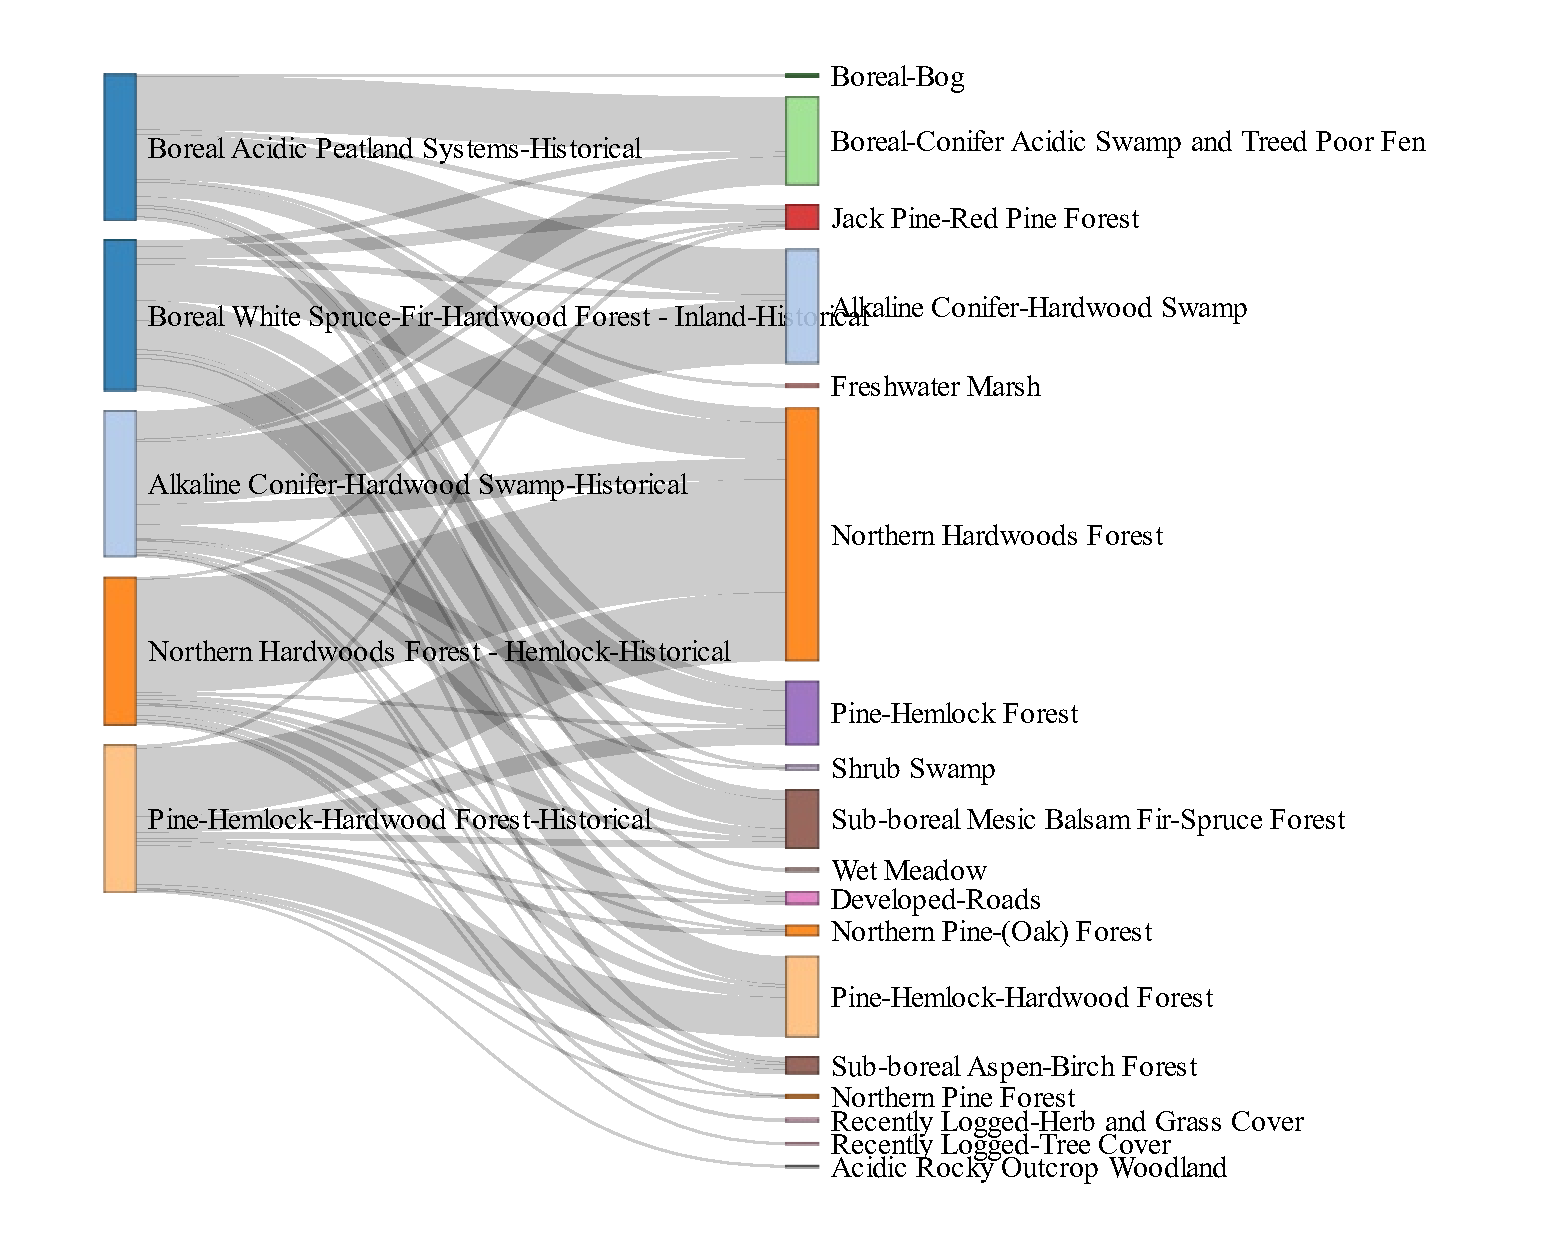
\includegraphics{FSCBook_files/figure-latex/sankey-1.pdf}

\hypertarget{successionClasses}{%
\chapter{Succession Classes}\label{successionClasses}}

\hypertarget{what-are-succession-classes}{%
\section{What are ``Succession Classes''?}\label{what-are-succession-classes}}

In general LANDFIRE succession classes are stages of development defined in the descriptions of each Biophysical Setting. They are characterized by height, canopy cover and to some degree species composition. Key takeaways:

\begin{itemize}
\tightlist
\item
  To learn what the succession classes are for each Biophysical Setting you look to the corresponding description on \url{http://landfirereview.org/test/search.php}
\item
  LANDFIRE used state and transition models to estimate the amount of each succession class that would occur with natural (pre-European colonization) disturbance regimes. Historical succession classes were not mapped as they were assumed to move around over time.
\item
  The \href{https://www.landfire.gov/sclass.php}{Succession Class} dataset maps current succession classes, in addition to agricultural and developed land-use classes plus uncharacteristic vegetation.
\item
  By comparing the amounts of historical and current succession classes you can get a sense of which classes are over/under represented.
\end{itemize}

\hypertarget{for-our-exercise-here}{%
\section{For our exercise here}\label{for-our-exercise-here}}

To illustrate the concept of comparing reference to current succession classes we will focus on

\hypertarget{histDist}{%
\chapter{Historical Disturbance Regimes}\label{histDist}}

Getting at historical disturbance regimes.

Need reviewed BpS model output spreadsheet.

\hypertarget{gisPrep}{%
\chapter{APPENDIX}\label{gisPrep}}

\hypertarget{gis-prep-combine-data}{%
\section{GIS Prep: Combine data}\label{gis-prep-combine-data}}

Once spatial data is properly projected and clipped to area of interest, perform a ``combine'' in ArcMap (Toolbox \textgreater{} Spatial Analyst \textgreater{} Local \textgreater{} Combine) of the BpS, SCL and EVT datasets. Alternatively, you can combine a raster of the area of interest with those 3 datasets which are stored as larger extents (like shown below).

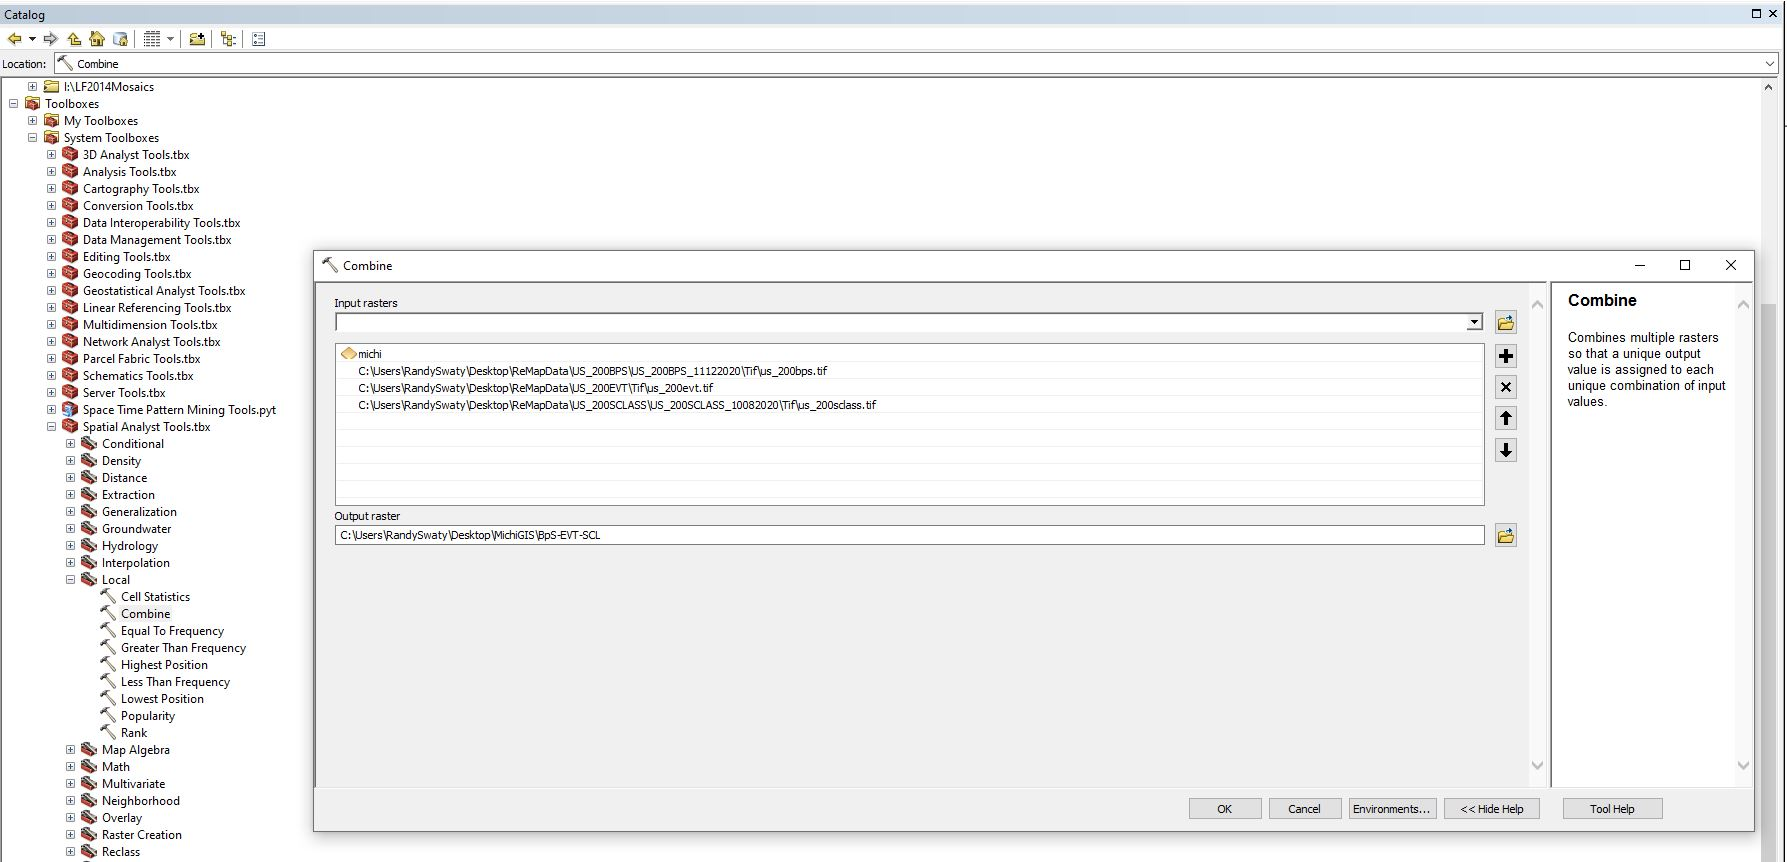
\includegraphics[width=1\linewidth]{combine}

\hypertarget{gis-prep-join-in-attributes}{%
\section{GIS Prep: Join in attributes}\label{gis-prep-join-in-attributes}}

There are multiple ways-we recommend using the Join Field tool (Toolbox \textgreater{} data management tools \textgreater{} joins \textgreater{} add join). One reason to do this is to be able to select which fields to join in. A potential resulting table looks like this for a landscape in Michigan (with minimal cleaning/formatting):

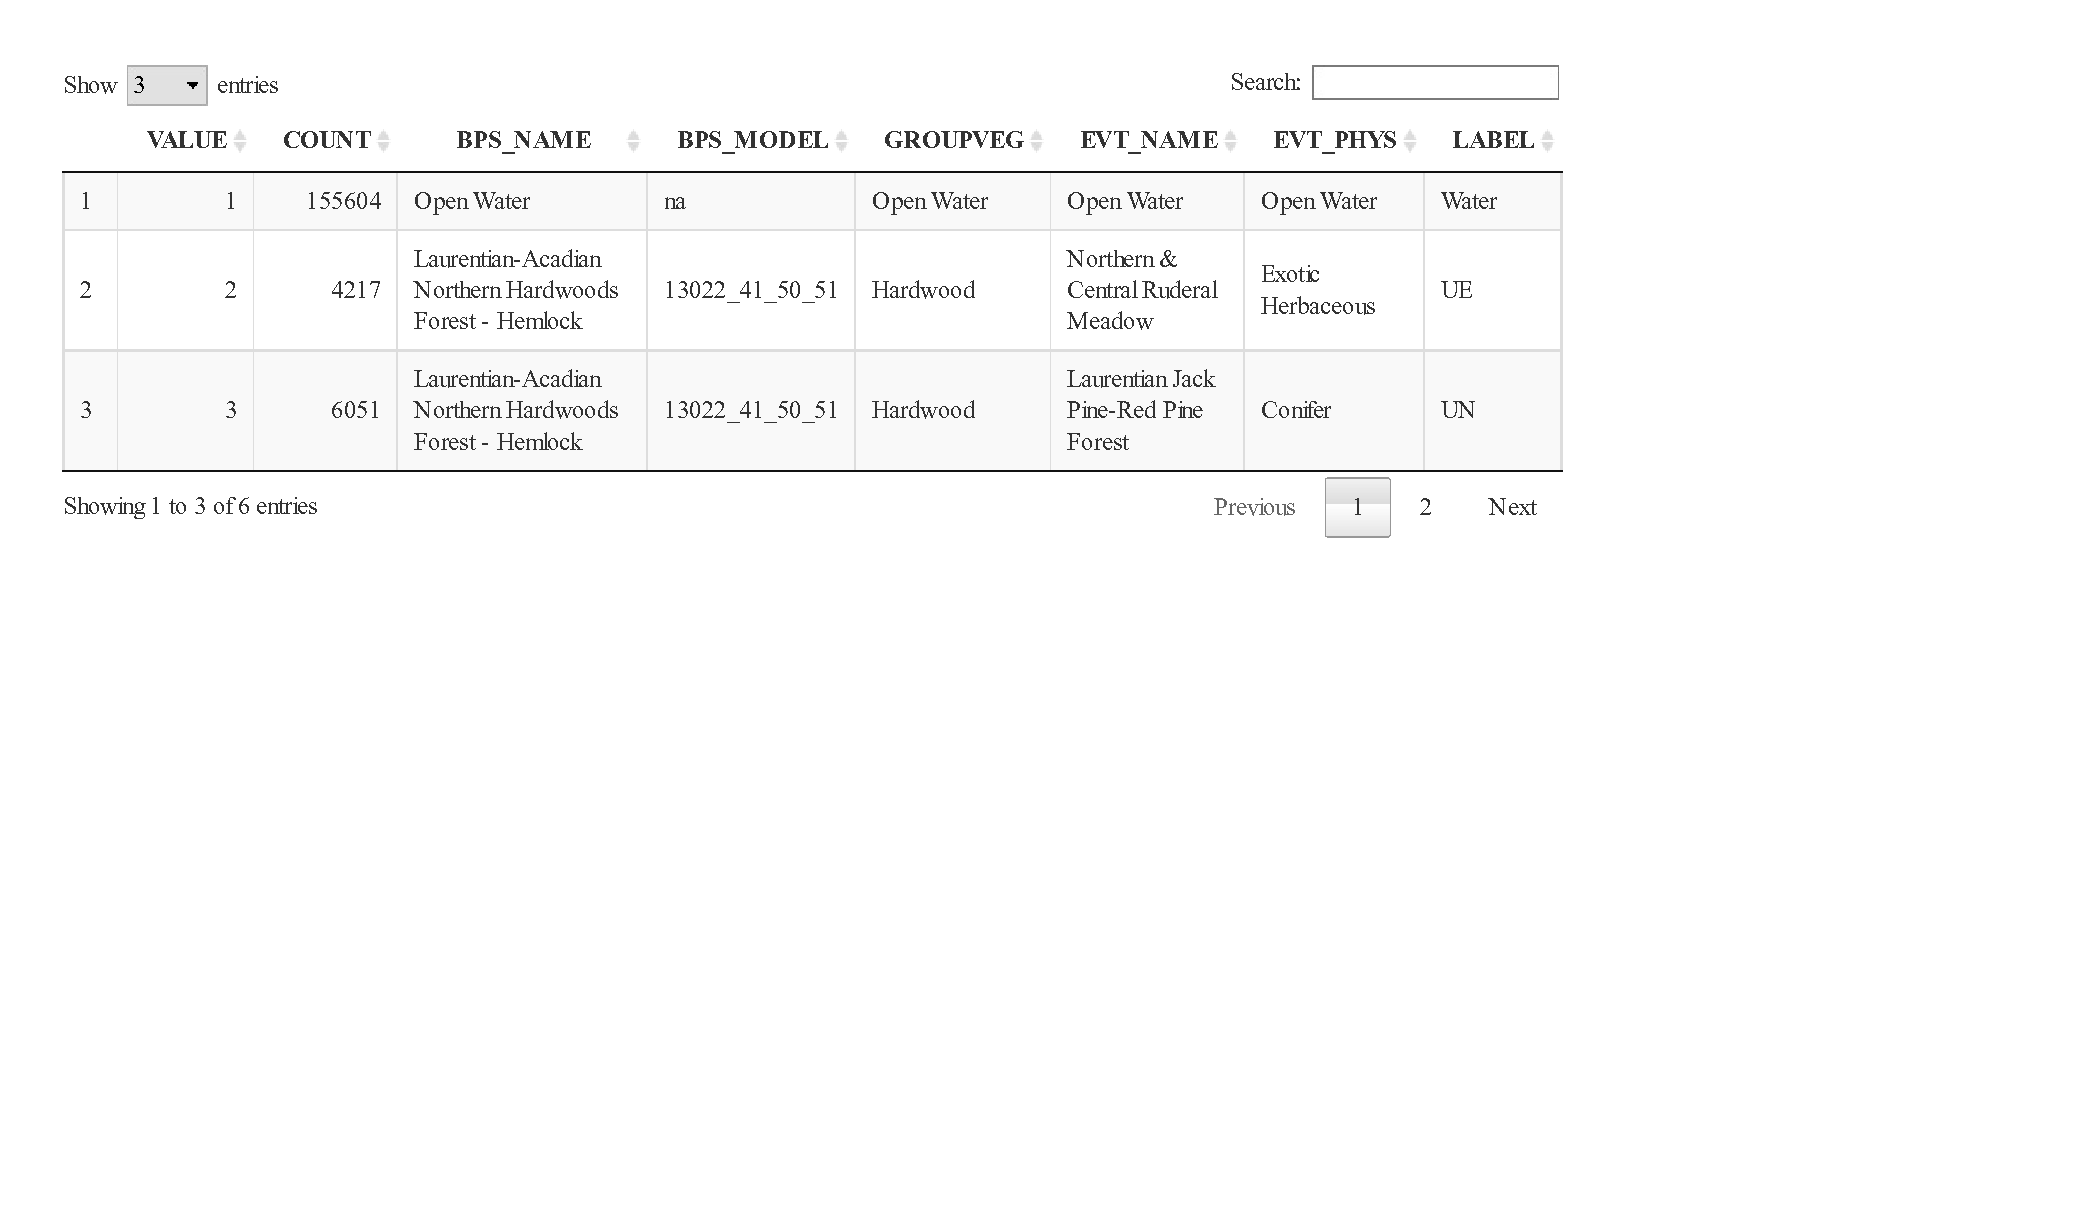
\includegraphics{FSCBook_files/figure-latex/combineDT-1.pdf}

As is this table does not mean too much-we will need to do some cleaning, formatting and calculating.

\hypertarget{gis-prepclean-data-table}{%
\section{GIS Prep:Clean data table}\label{gis-prepclean-data-table}}

You will first need to save the combined ``.csv'' file file as an ``.xlsx'' file so that you can have multiple worksheets. We recommend keeping the original output as a ``raw'' spreadsheet in Excel, pasting that data into a new sheet and working with that new sheet moving forward.
* It is OK to remove the ``US\_200BPS'', ``US\_200EVT'', and ``US\_200SCLASS'' columns
* Rename some columns: ``GROUPVEG'' to ``BPSGROUPVEG''; ``EVT\_PHYS'' to ``EVTGROUPVEG''; ``LABEL'' to ``SUCCESSIONCLASS'', or similar as needed for clarity
* COUNT = number of 30m x 30m pixels for that combination of BpS-EVT-SCLS. Insert a column named ``ACRES'', then calculate acres by multiplying COUNT by ``0.222''. Copy-Paste Values for that new column. Below is an example of what our new data table looks like.

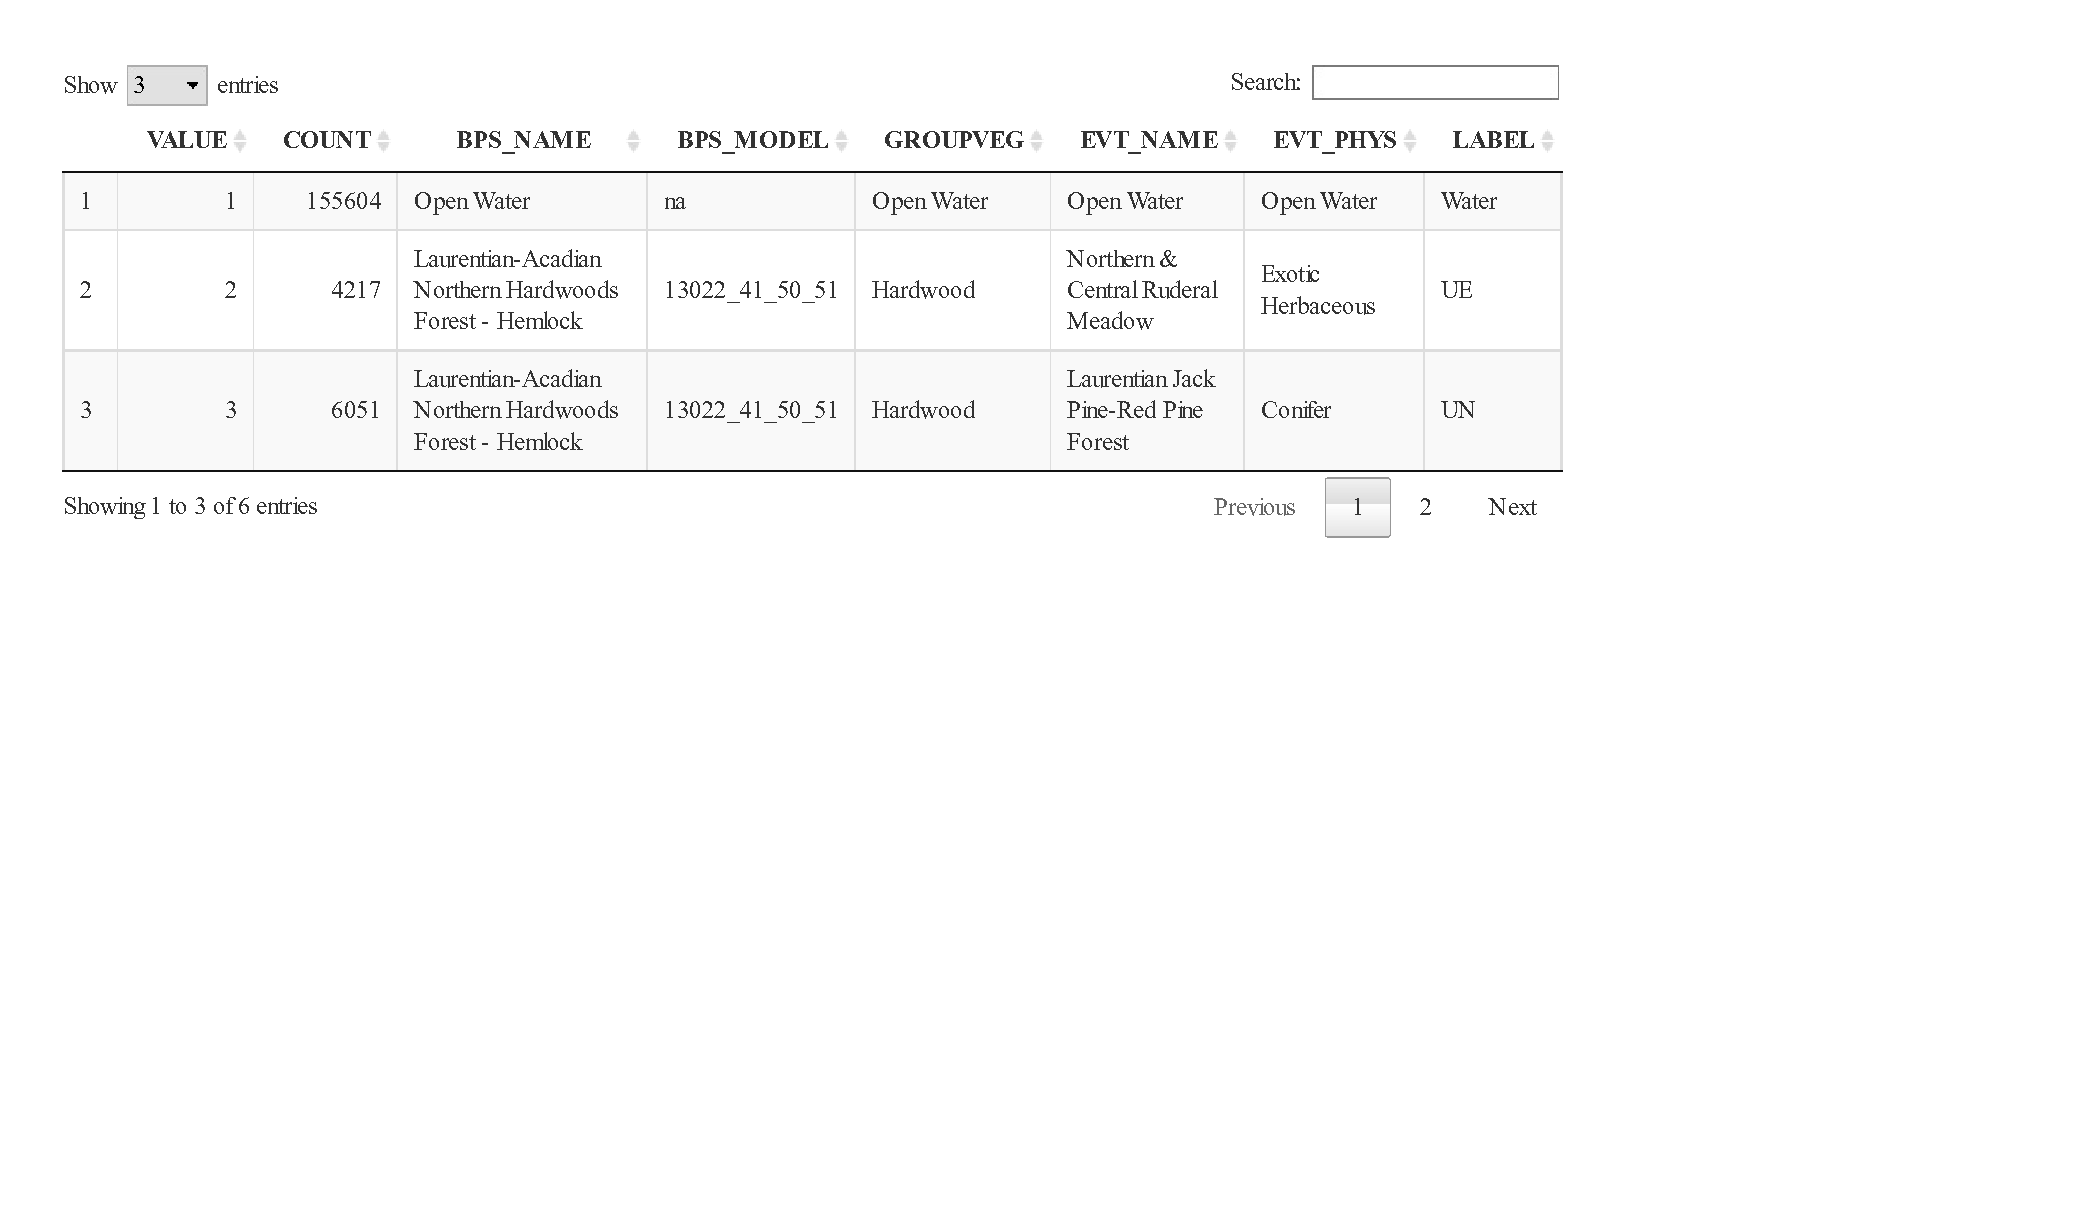
\includegraphics{FSCBook_files/figure-latex/combineCleanDT-1.pdf}

\hypertarget{final-words}{%
\chapter{Final Words}\label{final-words}}

We have finished a nice book.

HCVAs and RSAs:

HCVAs:

\begin{enumerate}
\def\labelenumi{\arabic{enumi}.}
\tightlist
\item
  High concentrations of biodiversity. G3 and above, s3 and above. Not individual species, but concentrations in the same area. Densities above average etc. compared to ecoregion. Multiple species.
\item
  Is there an area within or adjacent to an area legally designated by state or fed?\\
\item
  Does the FMU contain a known threatened or endangered species
\item
  Looking for ecological communities
\item
  outstanding areas
\end{enumerate}

RSA:

\begin{itemize}
\tightlist
\item
  places we have opportunities for progressive management
\item
  can we locate late successional? Issue will be species composition in LANDFIRE
\end{itemize}

\end{document}
